\chapter{Balança Comercial}
\section{Introdução}
\par A balança comercial define a diferença entre o registro de exportação de bens e serviços, adquiridos e vendidos de um país e a transação de compra de importação. Portanto, se o valor total das exportações for maior que o valor total das importações, o saldo é considerado positivo e também podemos chamá-lo de superávit comercial. Por outro lado, se as importações forem maiores que as exportações, haverá déficit ou saldo negativo. A balança comercial não considera a quantidade de produtos que entram ou saem de um país, mas sim os recursos gerados pela transação, o comportamento acompanha a balança comercial do Brasil e o Tocantins apresenta um saldo superavitário.

\section{Balança Comercinal de Janeiro a Junho de 2020}
\par No primeiro semestre de 2020(Jan-Jun), o estado do Tocantins atingiu um valor de US\$806,5 Milhões em exportações, valor correspondente à uma variação de 40,6\% em relação ao mesmo período de 2019, levando o estado a atingir o 16º lugar no país entre os maiores exportadores. 

\par Já os valores de produtos importados pelo estado neste mesmo período foi de US\$58,7 Milhões, o que representa uma variação negativa de -17,1\% em relação ao primeiro semestre de 2019, deixando o Tocantins na 25º posição no ranking nacional de importações por estados.

\par Sendo assim, o saldo total da balança comercial tocantinense no primeiro semestre de 2020 foi superavitário, à um valor de US\$747,8 Milhões. Dados estes, capazes de demonstrar que o estado do Tocantins têm uma balança comercial extremamente favorável, a cada ano se consolidando ainda mais como um estado considerado exportador.

\section{Produtos Exportados}
\subsection{Soja}

\par Representa 76\% do valor total de produtos exportados no primeiro semestre de 2020, a um valor US\$605 Milhões. De 2016 a 2018, a soja vinha apresentando constante aumento no valor e quantidade exportado nos primeiros semestres destes anos, mas a série foi interrompida por uma queda de de 21,5\% em 2019 em comparação a 2018. Em 2020 o valor voltou a subir, chegando a ser 32,9\% maior do que o mesmo período que no ano anterior.

\begin{figure}[h] 
	\caption{soja}
	\subcap{Em milhões de U\$}
	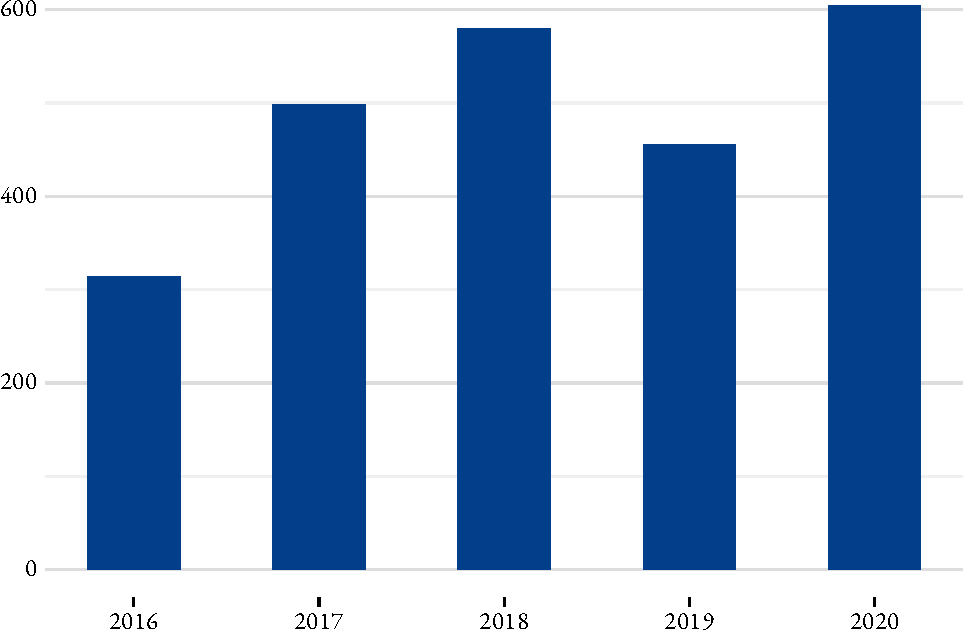
\includegraphics{fig/soja1-1.pdf}
	\source{COMEX STAT}
\end{figure}

\subsection{Carne Bovina(Fresca/Congelada ou Refrigerada)}
Correspondeu a 19\% do total exportado no primeiro semestre de 2020, atingindo o valor de US\$153 Milhões, o que significa crescimento de 125,6\% em relação ao mesmo período de 2019 onde o valor foi US\$67,8M. O histórico salto dos valores atingidos em 2020 podem significar uma nova fase para o futuro da carne bovina produzida no Tocantins ao se reafirmar como uma possível potência na produção e exportação deste produto no país.

\begin{figure}[h] 
	\caption{Carne Bovina/congelada ou refrigerada}
	\subcap{Em milhões de U\$}
	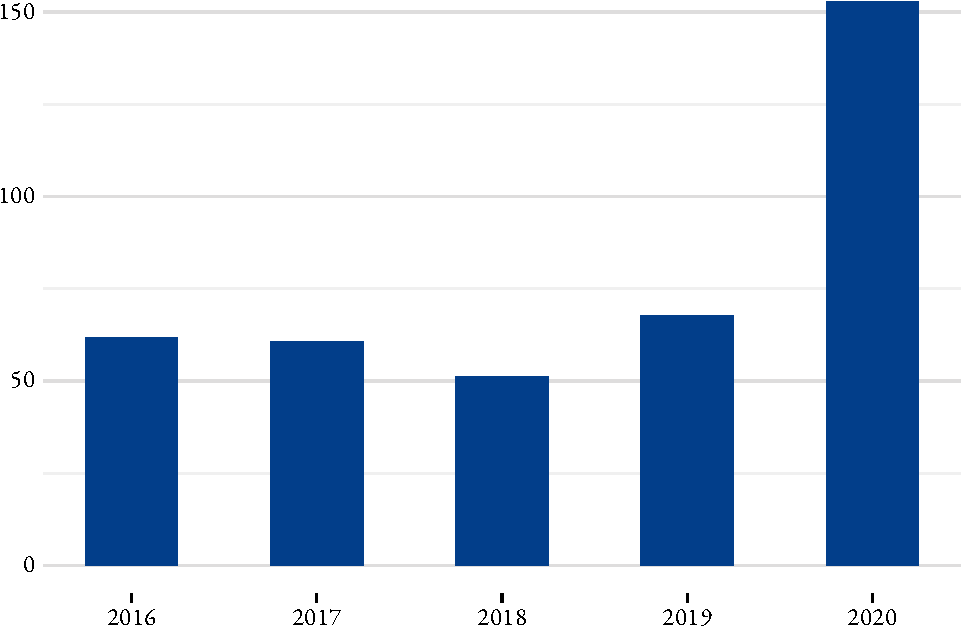
\includegraphics{fig/carne1-1.pdf}
	\source{COMEX STAT}
\end{figure}

\subsection {Farelos de soja e outros alimentos(excluídos cereais não moídos), farinhas de carnes e outros animais}
Responsável pela participação em 1\% das exportações estaduais no primeiro semestre de 2020, gerando um valor de US\$7,99M, mesmo ao sofrer uma considerável queda de 61,6\% do valor em relação ao mesmo período do ano anterior, estes produtos continuam sendo uma importante fonte de renda na agricultura estadual. 

\begin{figure}[h] 
	\caption{Farelos de Soja e Outros Alimentos (excluídos cereais não moídos), farinhas de carnes e outros animais}
	\subcap{Em milhões de U\$}
	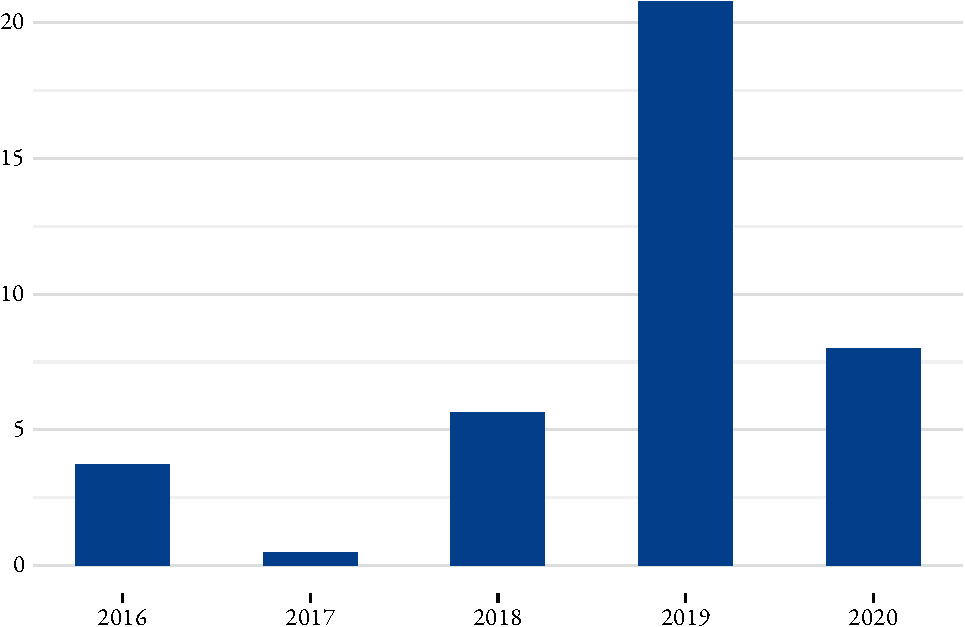
\includegraphics{fig/farelos1-1.pdf}
	\source{COMEX STAT}
\end{figure}

\subsection {Demais Produtos (Indústria de Transformação)}
\par Obtém uma participação de 0,91\% nos valores exportados no estado, ao valor de US\$7,17 Milhões, 18\% a menos do que o valor no mesmo período do ano anterior. Tais números não foram novidade para o setor, que vem demonstrando constante queda desde 2016 onde o valor exportado chegou a atingir US\$23,9 Milhões. A única exceção ocorreu no ano de 2019 onde o valor foi 3,2\% em relação ao de 2018. Estes dados demonstram que o foco das exportações tocantinenses ainda são, e cada vez mais se reafirmam nos produtos agrícolas, que estão em constantes crescentes, ao contrário dos produzido na indústria de transformação. 

\begin{figure}[h] 
	\caption{Demais Produtos (Indústria de Transformação}
	\subcap{Em milhões de U\$}
	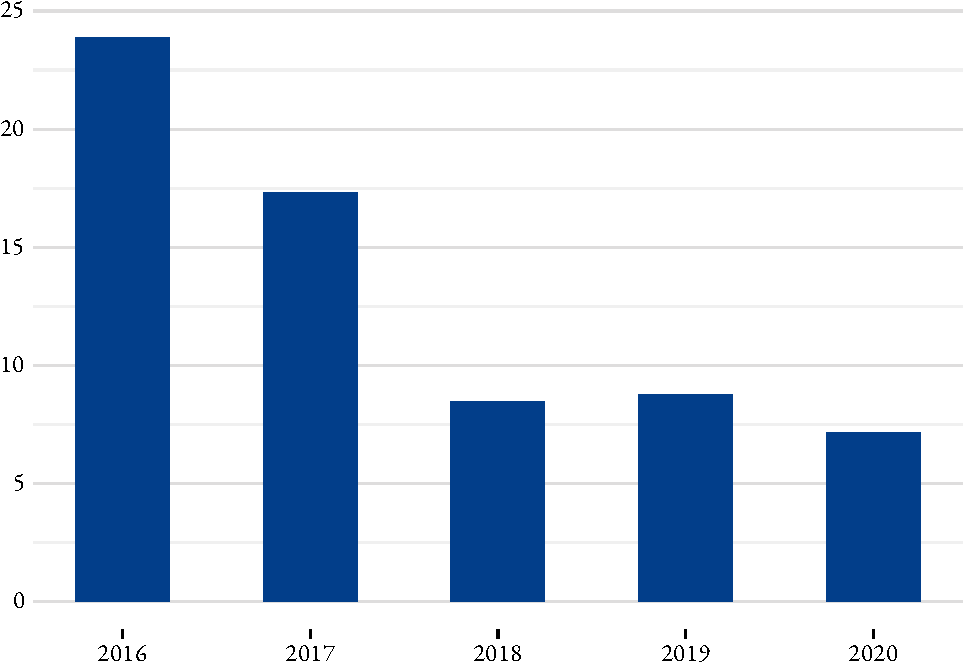
\includegraphics{fig/transf1-1.pdf}
	\source{COMEX STAT}
\end{figure}

\subsection{Matérias brutas de animais}
\par Têm uma participação de 0,88\% no total da exportação estadual, a um valor de US\$6,99 Milhões, valor este 11,5\% menor do que o arrecadado no mesmo período de 2019, ano onde houve o pico da exportação de matérias brutas de animais, atingindo US\$7,9 Milhões. Apesar da ligeira queda ocorrida este ano, o produto se mostra bastante estável na parte das exportações, com interessantes aumentos em relação a anos anteriores, se colocando como uma nova potência nas fontes de renda do estado.

\begin{figure}[h] 
	\caption{Matérias brutas de animais}
	\subcap{Em milhões de U\$}
	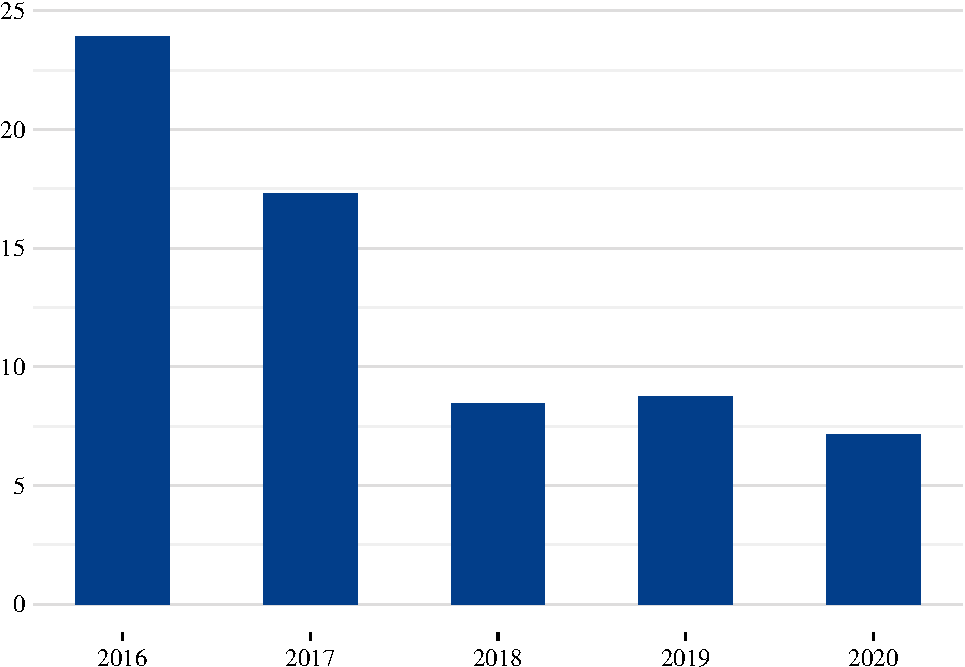
\includegraphics{fig/ultimo-1.pdf}
	\source{COMEX STAT}
\end{figure}

\section{Produtos Importados}

\subsection{Adubos ou fertilizantes químicos(exceto fertilizantes brutos)}
\par Obtém a maior participação nas importações do estado, sendo responsável por 53\% dos valores importados pelo tocantins no primeiro semestre deste ano. Apresenta uma série de crescimento constante nos últimos 5 anos, onde em 2020 atingiu um valor de US\$ 31,3 Milhões, significando um aumento de 7,7\% em relação ao mesmo período do ano passado.

\begin{figure}[h] 
	\caption{Adubos ou fertilizantes químicos(exceto fertilizantes brutos}
	\subcap{Em milhões de U\$}
	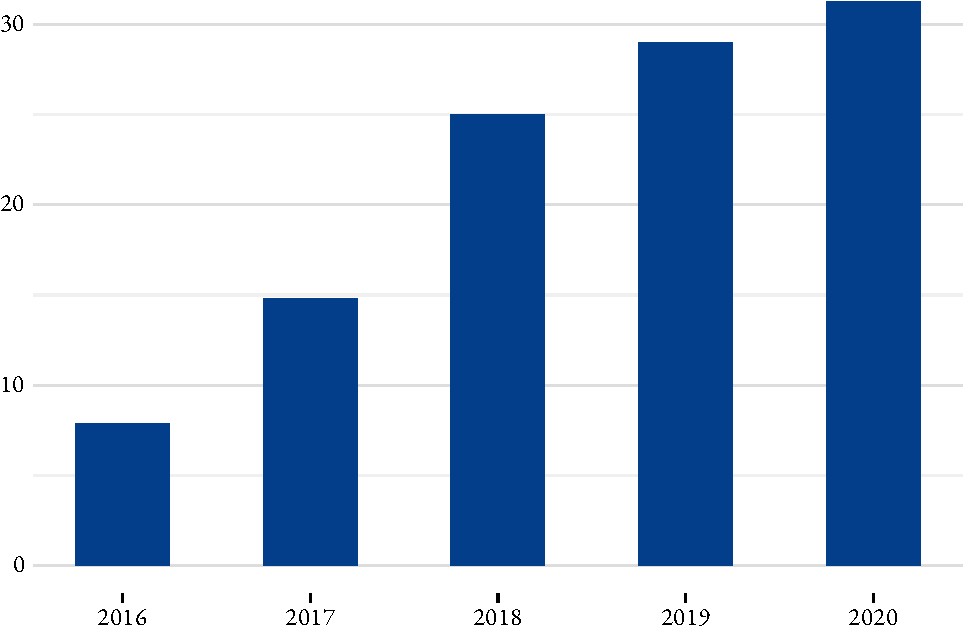
\includegraphics{fig/adubos1-1.pdf}
	\source{COMEX STAT}
\end{figure}

\newpage 

\subsection{Lentes e itens ópticos}
\par Após uma série de crescimento na importação de lentes e itens ópticos no primeiro semestre dos últimos dois anos, onde em 2019 atingiu seu pico à uma valor de US\$9 Milhões, em 2020 houve uma queda de 57,7\% em relação ao mesmo período do ano passado, sendo gastos apenas US\$3,80 Milhões na compra de materiais ópticos. 

\begin{figure}[h] 
	\caption{Lente e itens ópticos}
	\subcap{Em milhões de U\$}
	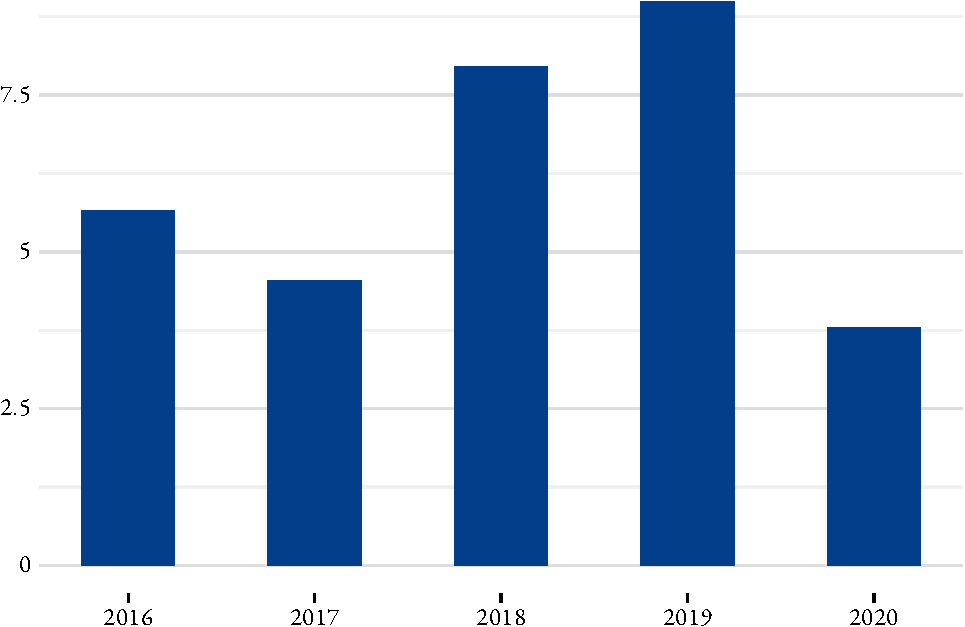
\includegraphics{fig/lentes1-1.pdf}
	\source{COMEX STAT}
\end{figure}

\subsection{Demais Produtos (Indústria de Transformação)}
\par Refere-se a 4,8\% do valor total das importações do estado. Após seguidas altas 2016 a 2018, Ano no qual atingiu o maior desempenho de sua participação na balança comercial tocantinense, a indústria de transformação apresentou consideráveis quedas nos anos seguintes, onde em 2020 atingiu seu menor índice na série histórica, sendo 46,6\% a menos que 2019 sendo um valor de US\$ 2,84 milhões. 

\begin{figure}[h] 
	\caption{Demais Produtos (Indústria de Transformação}
	\subcap{Em milhões de U\$}
	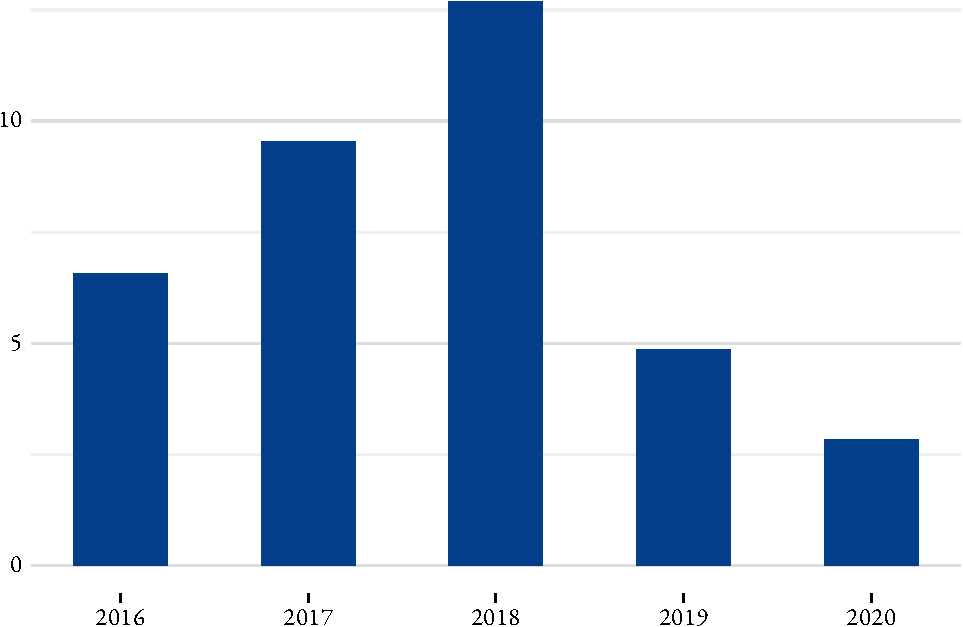
\includegraphics{fig/outros1-1.pdf}
	\source{COMEX STAT}
\end{figure}

\subsection{Óleos combustíveis de petróleo ou de minerais betuminosos(exceto óleos brutos)}
\par o apresentar um raro crescimento exponencial no ano de 2017 em comparação aos resultados de 2016, o produto apresentou três consecutivas quedas nos anos seguintes, atingindo em 2020 uma variação negativa 32,6\% sendo o valor US\$ 5,76 Milhões.

\begin{figure}[h] 
	\caption{Óleos combustíveis de petróleo ou de minerais betuminosos(exceto óleos brutos}
	\subcap{Em milhões de U\$}
	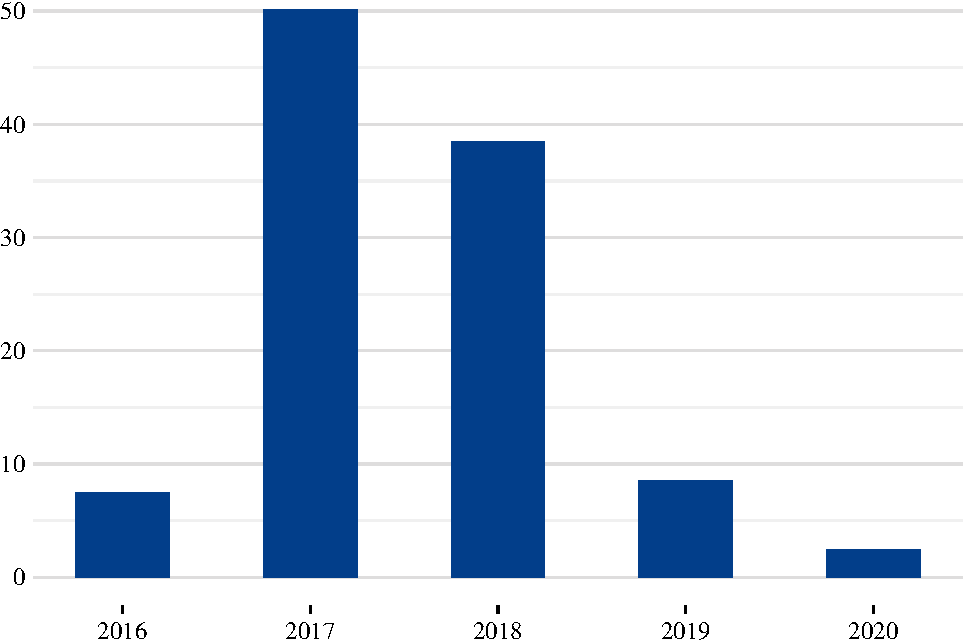
\includegraphics{fig/oleo-1.pdf}
	\source{COMEX STAT}
\end{figure}


\subsection{Instrumentos e aparelhos para usos medicinais, cirúrgicos, dentários ou veterinários}
\par Devido o novo coronavírus, SARS-COV-2, responsável pela pandemia de covid-19, que atingiu muitas pessoas simultaneamente ao redor do mundo no ano de 2020, o estado do Tocantins viu-se a necessidade de investir o equivalente a US\$2,45 Milhões na compra de produtos e equipamentos médicos para suprir a demanda de sua população este evento explica o aumento de 24000\% nos valores importados em relação ao mesmo período de 2019.

\begin{figure}[h] 
	\caption{Intrumentos e aparelhos para usos medicinais, cirúrgicos, dentários ou veterinários}
	\subcap{Em milhões de U\$}
	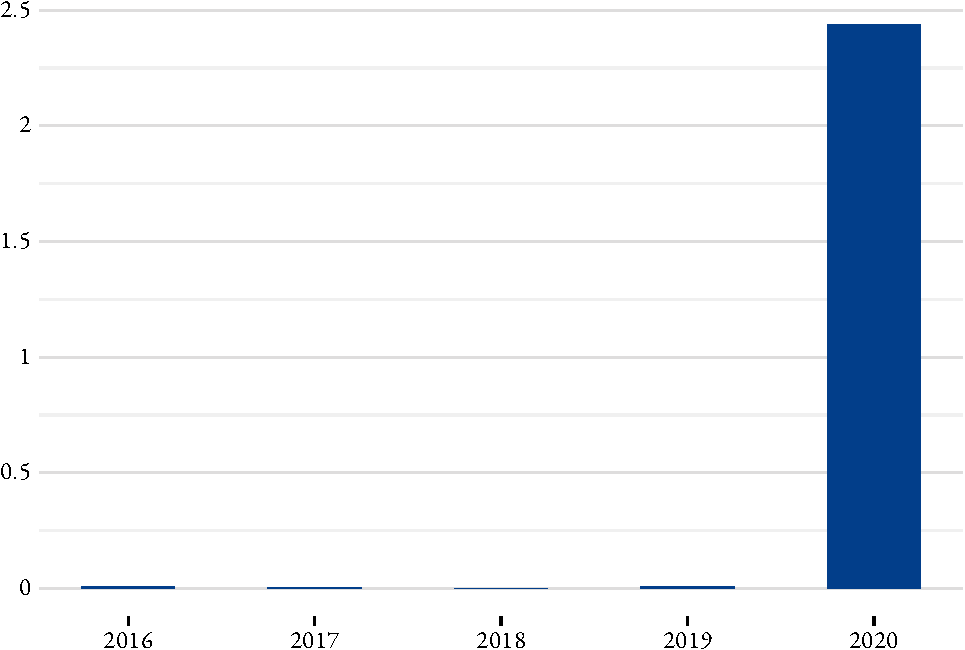
\includegraphics{fig/inst1-1.pdf}
	\source{COMEX STAT}
\end{figure}

\section{Países}
\par O Tocantins mantém relações comerciais com mais de 100 países ao redor do planeta, estabelecendo negócios em todos os continentes, seja com países potências na economia mundial, ou até mesmo com países de menor expressão no cenário econômico global. Essa diversidade de parceiros comerciais do estado é de extrema importância para que a expansão de suas divisas possa continuar trazendo benefícios para a economia tocantinense.

\subsection {Exportação}
\par Na tabela acima podemos ver o quão influente a China é nas exportações dos produtos tocantinenses, sendo responsável por 63\% do valor total exportado ano primeiro semestre de 2020. Este é um dos quesitos em que a balança comercial se assemelha à balança comercial brasileira, tendo a China como seu maior parceiro de exportações. 
A diversidade de países com relações comerciais com o Tocantins é visível na tabela, pois além da China, grande compradora dos grãos e carnes produzidos no estado, encontra-se também países como Espanha, representando 6,2\% do total exportado, Hong Kong, com 3,3\%; Bangladesh sendo 3,1\% e Rússia com 2,8\%

\subsection {Importação}
\par Em relação às importações, pode-se ver na tabela acima que a China também aparece como a principal parceira do estado, comprovando assim o tamanho de sua influência no saldo da balança comercial local, representando 31\% do total importado pelo estado no primeiro semestre de 2020, seguido pela Rússia com, 26\%, sendo os dois principais países dos quais o Tocantins compra produtos.. Mas em comparação à tabela de exportações, encontra-se mudanças, como a participação de países como Arábia Saudita, que foi responsável por 9,2\% das importações do Tocantins, sendo o terceiro principal parceiro nesta lista, seguido por México, com 4,6\% e República Tcheca com 4,1\%.

\section{Série Histórica de 2009 a 2019}

\subsection {Exportação 2009--2019}
\par As exportações do estado quase sempre se mantiveram em uma crescente, tendo
apenas dois anos em que o estado não obteve resultados positivos constantes. Em 2016 o estado teve seu maior declínio, saindo de US\$ FOB 901 milhões no ano de 2015, para US\$ FOB 633 milhões, uma variação negativa de  -29,8\%. 
Contudo em 2017 o Estado se recuperou com um crescimento de 50,3\%, e um valor de US\$ FOB 951. Em 2018 o Estado bateu recorde em exportação com um valor de US\$ FOB 1,2 Bilhões, mas não se mantendo constante em 2019 e perdendo 7,8\% desse valor em suas exportações.
No Acumulado de 10 anos o Estado conseguiu exportar US\$ FOB 8,106 Bilhões de dólares, com uma variação de 172,1\% de 2019 em relação à 2009.

\begin{figure}[h]
	\caption{Exportação}
	\subcap{Em bilhões de U\$}
	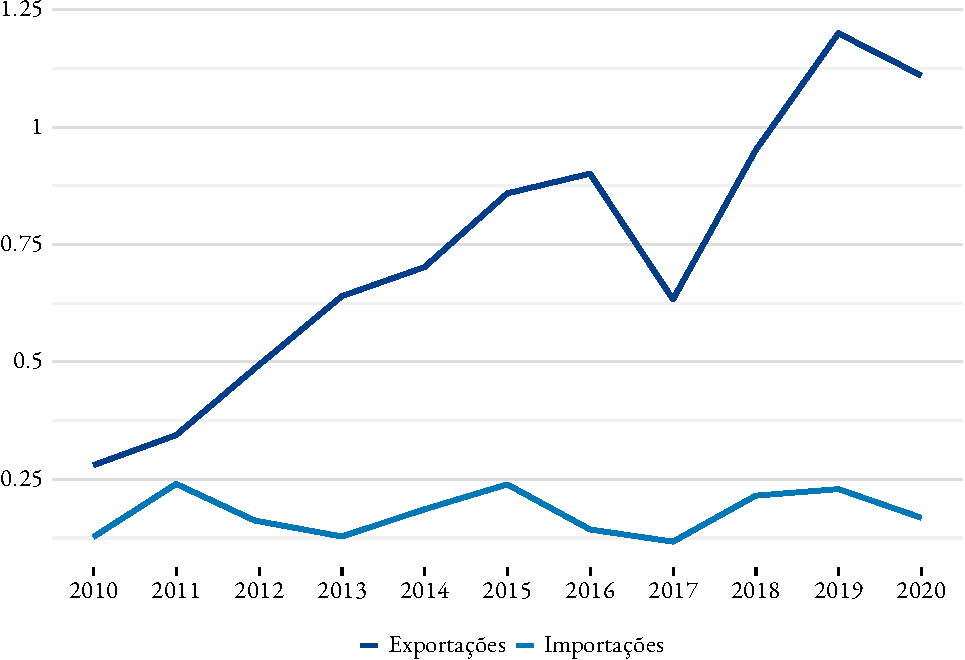
\includegraphics{fig/total-1.pdf}
	\source{COMEX STAT}
\end{figure}

\subsection{Importação 2009--2019}
\par Os valores das importações do Tocantins de 2009 à 2019 apresentam falta de estabilidade em seu crescimento, seguido um padrão de 2 anos de crescimento e 2 anos de baixa em seus valores importados. Enquanto em 2010 apresentou um valor recorde de variação na importação no período analisado de 88,4\%, e também um valor bruto superior aos outros 9 anos, com US\$ FOB 240 milhões de importados.

\subsection{Saldo 2009--2019}

\par Historicamente o Tocantins apresenta sempre um saldo superavitário em sua balança comercial, onde o menor valor dos últimos 10 anos foi uma expressiva marca de de US\$ 104 milhões ainda em 2009. Já seu valor recorde foi de US\$ 975 milhões de dólares no ano de 2018, ano este onde o estado atingiu sua máxima histórica nos valores de exportação

\begin{figure}[h]
	\caption{Saldo}
	\subcap{Em bilhões de U\$}
	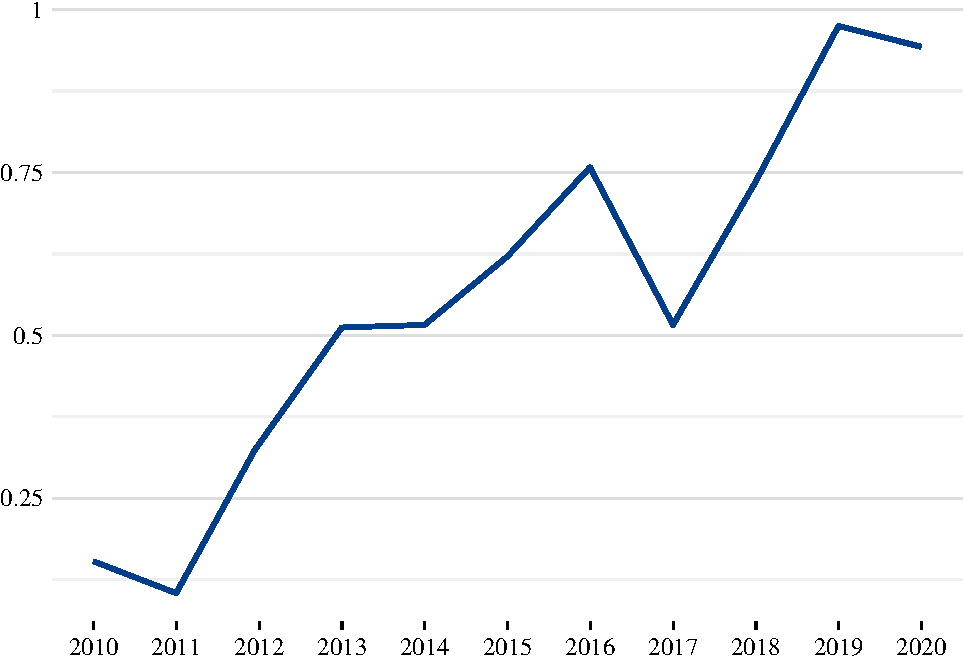
\includegraphics{fig/sal1-1.pdf}
	\source{COMEX STAT}
\end{figure}

\par De 2010 à 2019 o estado tem um saldo acumulado de US\$ 6,1 bilhões, com uma variação de 320,6\% deste período. Tais dados mostram o potencial do estado em adquirir riqueza exportando seus produtos. 
